\documentclass[10pt]{beamer}

\usepackage[T1]{fontenc}
\usepackage[utf8]{inputenc}
\usepackage[frenchb]{babel}
\usepackage{eurosym}

\usepackage{graphicx}


\newcommand\host{{\it host}\,}
\newcommand\device{{\it device}\,}



% --------- BEGIN STYLE BEAMER ---------
\usetheme{Madrid}
\definecolor{ECNBleu}{HTML}{102648}
\definecolor{ECNJaune}{HTML}{FAB600}

\setbeamercolor{frametitle}{bg=ECNBleu,fg=white} %le titre de la frame, en haut
\setbeamercolor{title in head/foot}{bg=ECNJaune,fg=ECNBleu} %barre bas, milieu
\setbeamercolor{author in head/foot}{bg=ECNBleu,fg=ECNJaune} %barre bas, gauche
\setbeamercolor{date in head/foot}{bg=ECNBleu,fg=ECNJaune} %barre bas, droit
\setbeamercolor{section in head/foot}{bg=ECNJaune,fg=ECNBleu} %haut gauche
\setbeamercolor{subsection in head/foot}{bg=ECNBleu,fg=ECNBleu} %haut droite
\setbeamercolor{title}{bg=ECNBleu,fg=white}
\setbeamercolor{block title}{fg=white,bg=ECNBleu}

%\setbeamercolor{normal text}{bg=IUTBleuFonce} %texte
\setbeamercolor{item}{bg=ECNBleu}
\setbeamercolor{subitem}{bg=ECNJaune}
\setbeamercolor{description item}{fg=couleurEmph}
\setbeamercolor{section in toc}{fg=ECNBleu}
%\setbeamercolor{subsubitem}{bg=IUTBleuFonce}

%structure (eq emph dans beamer)
\setbeamercolor{emph}{fg=couleurEmph}
% ----------------------------

\usepackage{listings}

\lstdefinestyle{customc}{
  belowcaptionskip=1\baselineskip,
  breaklines=true,
  frame=L,
  xleftmargin=\parindent,
  language=C,
  showstringspaces=false,
  basicstyle=\tiny\ttfamily,
  keywordstyle=\bfseries\color{green!40!black},
  commentstyle=\itshape\color{purple!40!black},
  identifierstyle=\color{blue},
  stringstyle=\color{orange},
}

\lstset{escapechar=@,style=customc}

\newenvironment<>{questionblock}[1]{%
\setbeamercolor{block title}{bg=ECNJaune,fg=ECNBleu}%
\begin{block}#2{#1}}{\end{block}}

\title[GPGPU]{Programmation sur Processeur Graphique}

\subtitle[\ldots]{
---\\Partie 6 : Utilisation des ressources d'exécution}
\author[P.-E. Hladik]{Pierre-Emmanuel Hladik\\\tiny pierre-emmanuel.hladik@ec-nantes.fr}
\institute[Centrale Nantes]{}
\date{\today}

\begin{document}

 \frame{\titlepage}


%https://oneflow2020.medium.com/how-to-choose-the-grid-size-and-block-size-for-a-cuda-kernel-d1ff1f0a7f92
%%%%%%%%%%%%%%%%%%%%%%%%%%
\begin{frame}[plain]
\frametitle{Unité d'exécution : Streaming Multiprocessors}

	\begin{itemize}
		\item Les unités de calculs sont des {\bf Streaming Multiprocessors} (SM)
		\item Chaque SM dispose d'un nombre de cœurs à allouer pour les calculs
		\item Un cœur exécute un thread
	\end{itemize}
	\bigskip
	
	\begin{block}{Exemple Jetson Nano : Maxwell GPU}
128-core GPU | End-to-end lossless compression | Tile Caching | OpenGL$^{\text{\tiny ®}}$ 4.6 | OpenGL ES 3.2 | VulkanTM 1.1 | CUDA$^{\text{\tiny ®}}$ | OpenGL ES Shader Performance (up to): 512 GFLOPS (FP16)
Maximum Operating Frequency: 921MHz
	\end{block}

\end{frame}
%%%%%%%%%%%%%%%%%%%%%%%%%%
\begin{frame}[plain]
\frametitle{Exécution des {\it blocks}}

	\begin{itemize}
		\item L'exécution des calculs est géré au niveau des {\it blocks}
		\item Les {\it blocks} sont affectés sur n'importe quel SM
		\item Un SM peut exécuter plusieurs {\it blocks} s'il y a assez de ressources
		\item Un {\it block} s'exécute entièrement sans être interrompu
		\item Un {\it block} s'exécute dans n'importe quel ordre par rapport aux autres
	\end{itemize}
      \center
	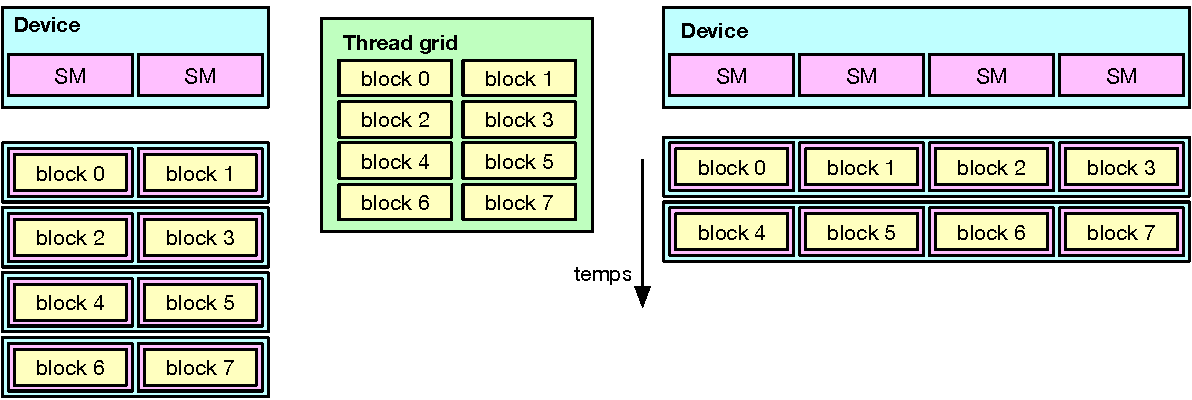
\includegraphics[width=\textwidth]{./figures-pdf/scalability}

\end{frame}

%%%%%%%%%%%%%%%%%%%%%%%%%%
\begin{frame}[plain]
\frametitle{Contrôleur d'exécution : Warp}

	\begin{block}{Problème}
	Usuellement il y a plus de threads que de coeurs dans un SM. Le système doit donc choisir l'ordre dans lequel les threads sont exécutés, c'est un {\bf problème d'ordonnancement}
	\end{block}

	\begin{itemize}
		\item Le flot d'exécution des threads est contrôlé par les {\bf Warps}
		\item Un warp est un groupe de 32 threads d'index consécutifs (i.e. leur threadIdx -- les thread 0 à 31 forment le premier warp, 32 à 63 le second, etc.). Le nombre peut varier en fonction des architectures, mais ne se choisit pas logiciellement.
		\item Si le nombre de threads n'est pas un multiple de 32, certains coeurs alloués au Warp ne font rien.
		\item Les threads d'un warp s'exécutent en SIMD (à tout moment, une instruction est récupérée (fetch) et exécutée (dispatch) pour tous les threads), c'est-à-dire que tous les threads d'un warp exécutent la même instruction sur différentes données.
		\item Tous les threads d'un warp ont le même temps d'exécution
	\end{itemize}

\end{frame}


%%%%%%%%%%%%%%%%%%%%%%%%%%
\begin{frame}[plain]
\frametitle{Ordonnancement des warps}


	\begin{itemize}
		\item Les warps sont les unités d'ordonnancement dans un SM
		\item Un warp qui attend le résultat d'une opération avec une longue latence libre le SM (pour ne pas bloquer le SM)
		\item Un autre warp dont une instruction est prête à s'exécuter est choisi
		\item Si plus d'un warp est prêt à être exécuté, un mécanisme de priorité est utilisé pour en sélectionner un
	\end{itemize}
	
		\begin{block}{}
		Cette politique d'ordonnancement est appellée  {\bf Zero-overhead thread}, elle évite d'introduire des temps morts et fait au mieux pour utiliser les ressources d'exécution.
	\end{block}
	
	\begin{alertblock}{}
		Mise en pratique...
	\end{alertblock}

\end{frame}

%%%%%%%%%%%%%%%%%%%%%%%%%%
\begin{frame}[plain]
\frametitle{Performances}

	\begin{itemize}
		\item Cet ordonnancement permet de combler les temps morts dûs aux latences des opérations en choisissant les warps/threads qui peuvent s'exécuter au plus tôt. Ce mécanisme est appelé \og latency tolerance \fg \,ou \og latency hiding \fg\, (similaire à la gestion d'un guichet à la poste)\medskip
		\item Entrelace efficacement les opérations avec des longues latences, comme les accès globaux à la mémoire, les instructions arithmétiques à virgule flottante, etc.
	\end{itemize}

\end{frame}


%%%%%%%%%%%%%%%%%%%%%%%%%%
\begin{frame}[plain]
\frametitle{Optimiser les performances}

	\begin{block}{Définition : taux d'occupation}
		Le rapport entre le nombre de threads en cours d'exécution sur le SM et le nombre maximum de threads que peut prendre en charge un SM est appelé le {\bf taux d'occupation} {\it occupancy}. 
	\end{block}

\vspace{1em}

	Plus le taux d'occupation est élevé, plus les performances potentielles sont importantes.
	
	\begin{block}{Problème}
		Comment maintenir un nombre suffisant d'instructions dans le pipeline en même temps ? Sachant que le seul paramètre logiciel sur lesquel jouer est le nombre de threads par block (et réciproquement le nombre de blocks).
	\end{block}
	
	Voir : \href{https://docs.nvidia.com/cuda/cuda-c-programming-guide/index.html\#performance-guidelines}{Nvidia Performance guidelines}

\end{frame}

%%%%%%%%%%%%%%%%%%%%%%%%%%
\begin{frame}[plain]
\frametitle{Règles intuitives pour dimensionner les blocks}

	\begin{block}{Première régle : multiple du nombre de threads par warp}
		Le nombre de threads par block doit être choisi comme un multiple du nombre de threads par warp afin d'éviter autant que possible de gaspiller des ressources de calcul avec des warps sous-utilisés.
	\end{block}
	
		\begin{block}{Seconde règle : beaucoup de warps}
		Il faut suffisamment de warps pour que le matériel trouve un warp à exécuter à tout moment, ce qui permet d'utiliser pleinement le matériel d'exécution malgré des opérations avec des latences longues... mais attention, s'il y a des warps longs, le block devra attendre la terminaison de tous les warps avant de rendre la main.
	\end{block}

\end{frame}
%%%%%%%%%%%%%%%%%%%%%%%%%%
\begin{frame}[plain]
\frametitle{Contraintes sur les ressources d'exécution}

Les ressources d'exécution sont limitées par :
		\begin{itemize}
		\item {\bf le nombre de coeurs} de l'architecture qui limite le nombre de threads pouvant être exécuté simultanément (le SM Jetson Nano NVIDIA Maxwell dispose de 128 coeurs NVIDIA CUDA)
		\item {\bf le nombre maximum de blocks résidents} par SM (32 Jetson Nano)
		\item {\bf le nombre maximum de warps résidents} par SM (64 Jetson Nano)
		\item {\bf le nombre maximum de threads résidents} par SM (2048 Jetson Nano), c'est-à-dire le nombre maximum de blocks et de threads qui peuvent être exécutés simultanément sur le SM.
		\end{itemize}

\end{frame}
%%%%%%%%%%%%%%%%%%%%%%%%%%
\begin{frame}[plain]
\frametitle{Contraintes sur la mémoire}

Les performances dépendent aussi des ressources mémoires :
	\begin{itemize}
		\item la quantité totale de {\bf mémoire partagée} est limitée par :
		\begin{itemize}	
			\item la quantité maximale de mémoire partagée par SM (64ko pour la Jetson Nano)
			\item la quantité maximale de mémoire partagée par block de threads (48ko)
		\end{itemize}
		\medskip
		\item la quantité totale de {\bf registres} est limitée par :
		\begin{itemize}	
			\item Nombre de registres 32 bits par SM (64 000 pour la Jetson Nano)
			\item Nombre maximal de registres 32 bits par block de threads (32 000)
			\item Nombre maximal de registres 32 bits par thread (255)
		\end{itemize}

	\end{itemize}

	\begin{block}{}
		Le nombre de registres utilisés par un kernel peut avoir un impact significatif sur le nombre de warps résidents.
	\end{block}

%Le fichier de registres est organisé en registres de 32 bits. Ainsi, chaque variable stockée dans un registre nécessite au moins un registre de 32 bits, par exemple, une variable double utilise deux registres de 32 bits.

L'utilisation des registres et de la mémoire partagée est retourné par le compilateur avec l'option {\tt -{}-ptxas-options=-v}

\end{frame}
%%%%%%%%%%%%%%%%%%%%%%%%%%
\begin{frame}[plain]
\frametitle{Alors comment optimiser les performances ?}


		\begin{block}{Conclusion}
The effect of execution configuration on performance for a given kernel call generally depends on the kernel code. {\bf Experimentation is therefore recommended.}  [\href{https://docs.nvidia.com/cuda/cuda-c-programming-guide/index.html\#overall-performance-optimization-strategies}{documentation Nvidia}]
		\end{block}

\end{frame}



%%%%%%%%%%%%%%%%%%%%%%%%%%%
%\begin{frame}[plain]
%\frametitle{Petit exemple}
%
%Supposons qu'un \device autorise jusqu'à 8 blocks par SM, 1024 threads par SM et 512 threads par block.
%
%\begin{block}{}
%	Pour traiter une image doit-on utiliser des blocks de 8×8, 16×16, ou 32×32 threads ?
%\end{block}
%
%
%	\begin{itemize}
%	\only<1>{
%		\item 8x8 : chaque block a 64 threads. %Nous aurons besoin de 1024/64 = 12 blocks pour occuper entièrement un SM. 
%		Cependant, un SM ne peut accueillir que 8 blocks ; nous n'aurons donc que 64 × 8 = 512 threads dans chaque SM (ou exécuté les uns après les autres s'il n'y a qu'un SM). Ce nombre implique qu'un block aura 64/32= 2 warps et 
%		que les ressources d'exécution des SM seront probablement sous-utilisées car il y aura peu de warps disponibles pour planifier les opérations avec de longues latences.
%		}
%	\only<2>{
%		\item 16x16 : il ya 256 threads par block, ce qui implique l'utilisation de 4 blocks. Ce nombre est dans la limite des 8 blocks par SM. Il y aura au total et est une bonne configuration car il nous permet d'avoir une capacité de threads complète dans chaque SM et un nombre maximal de warps pour l'ordonnancement. 
%		}
%	\only<3>{
%		\item 32x32 : Les blocks 32×32 donneraient 1024 threads dans chaque block, ce qui dépasse la limite de 512 threads par block de ce \device.
%		}
%	\end{itemize}
%
%
%\end{frame}


\end{document}